\section{Theoretical Analysis}
\label{sec:analysis}


In these section we represent the plots that were produced by our theoretical analysis. These plots represents the Voltage on Envelope Detector and the output voltage of the circuit.

\begin{figure} [!htb] 
  \minipage{0.9\textwidth}
  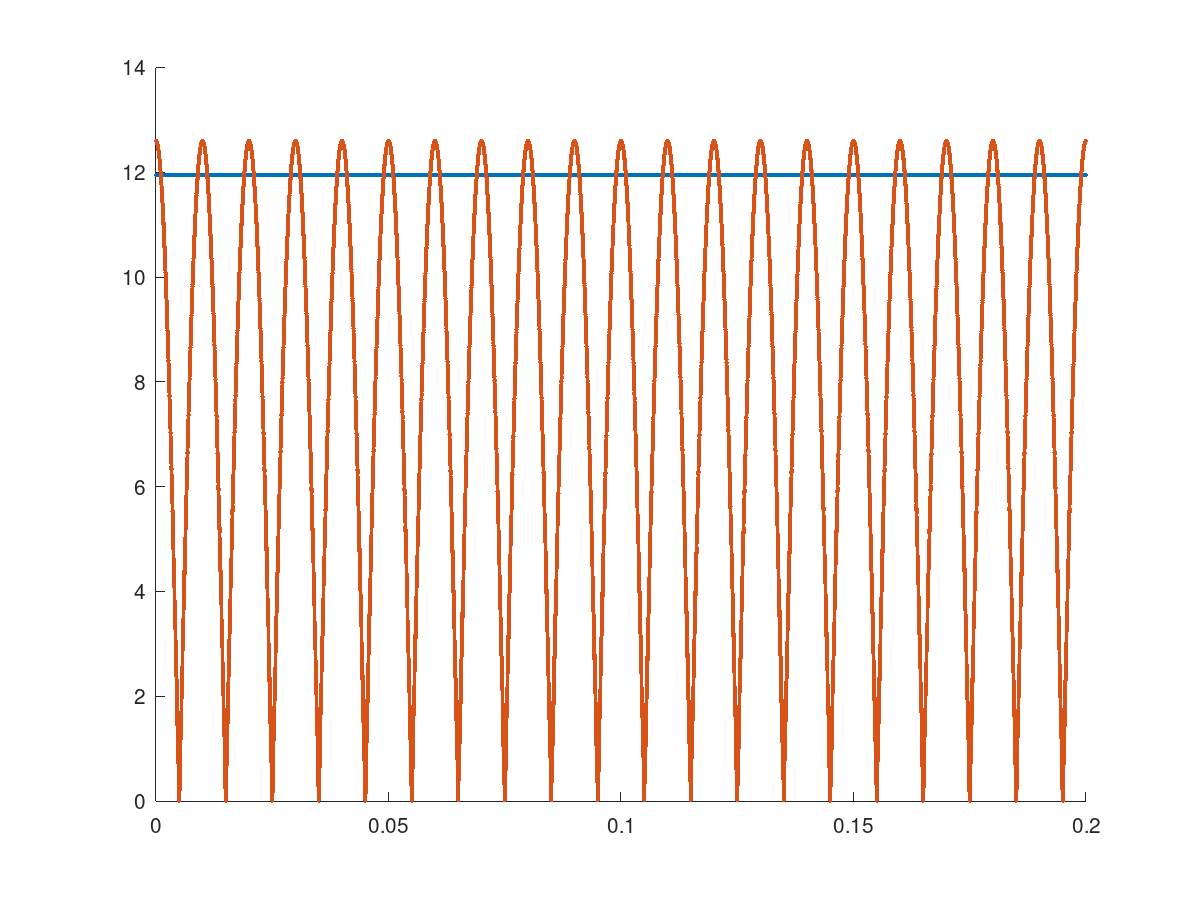
\includegraphics[width=\linewidth]{Condensador.png}
  \caption{Envelope Detector and Output Voltages}
  \label{fig:theoplots}
  \endminipage\hfill
\end{figure}

To produce these plots we considered a diode model composed of a DC voltage source, resistor, and ideal diode, and ran a mathematical analysis of the components of the circuit that were active at that time.\\
To run the analysis itself, we created two mathematical models, one where the diodes were off, and one where they were on. We then ran the calculations for each timestep and used "if" statements to switch between the conducting and non conducting modes of the diodes in function of the voltage across them. In the end, due to the design we picked, it worked out to be indifferent wether or not we did this, since the resistance of the voltage limiter when it is off is infinite in our model, the capacitor never discharges, the ripple is zero, and the average voltage is exactly 12.


\FloatBarrier
\begin{table}[h]
  \centering
  \begin{tabular}{|c|c|}
    \hline    
    
 $V_{ripple}$ & $V_{DC}$ \\ 
 2.61313e-05 V   & 11.95 V\\

    \hline
  \end{tabular}
  \caption{Ripple and DC voltages}
  \label{tab:Octave}
\end{table}
\FloatBarrier 

\begin{equation}
  frac{v_o}{v_i} = -g_{m}(frac{1}{R_C}+frac{1]{r_o})v_{pi}
  \label{}
\end{equation}  


%\par According to the conventional way, the transformers wires are coiled, so assuming that, in order to produce a downwards current through the Tranformer 1 and an upwards current through the Transformer 2, we have the correlation that:

%\begin{equation}
%  V_(t1)= n*V_(t2)
%  \label{}
%\end{equation}    

%where $n$ is the number of turns seen in Transformer 1; $V_(t1)$ is the AC signal in Transformer 1; V_(t2) is the signal in Transformer 2.  

%\par Because the objective is to obtained a DC voltage of 12V in the output, a sinusoidal signal of amplitude $qq coisa não esquecer$ was used for transformer number 2. 

%\par Due to (a certain number of diodes) in the full-wave bridge rectifier circuit, the voltage through resistance $R_1$ can be compute as: 

%\begin{equation}
 % V_(0_(rect))=|V_(t2)|
%  \label{}
%\end{equation}    

%For these theoretical analysis an ideal diode model has been considered and a capacitor, who is in charge to keep the volatge mainly constant and close to 12V. For that matters the time that it takes to the diode circuit to go OFF and for the capacitor to start discharging through the $R_1$ is given by: 

%\begin{equation}
%  V_(0_(rect))=|V_(t2)|
%  \label{}
%\end{equation}    
